A ``spacer plate'' with a peg attaches the drone arms to the body with perfect-fit contact only.
Since the drone will not experience high G-forces or intense maneuvers, this attachment is not supplemented by screws or glue.
Screws attach the Raspberry Pi, power distribution board, and motors to the drone body.
The electronic speed controllers and their wires are secured in their mounts by tape.
The assembled drone is shown in Figure \ref{figure:drone_assembled}.

\begin{figure}
    \centering
    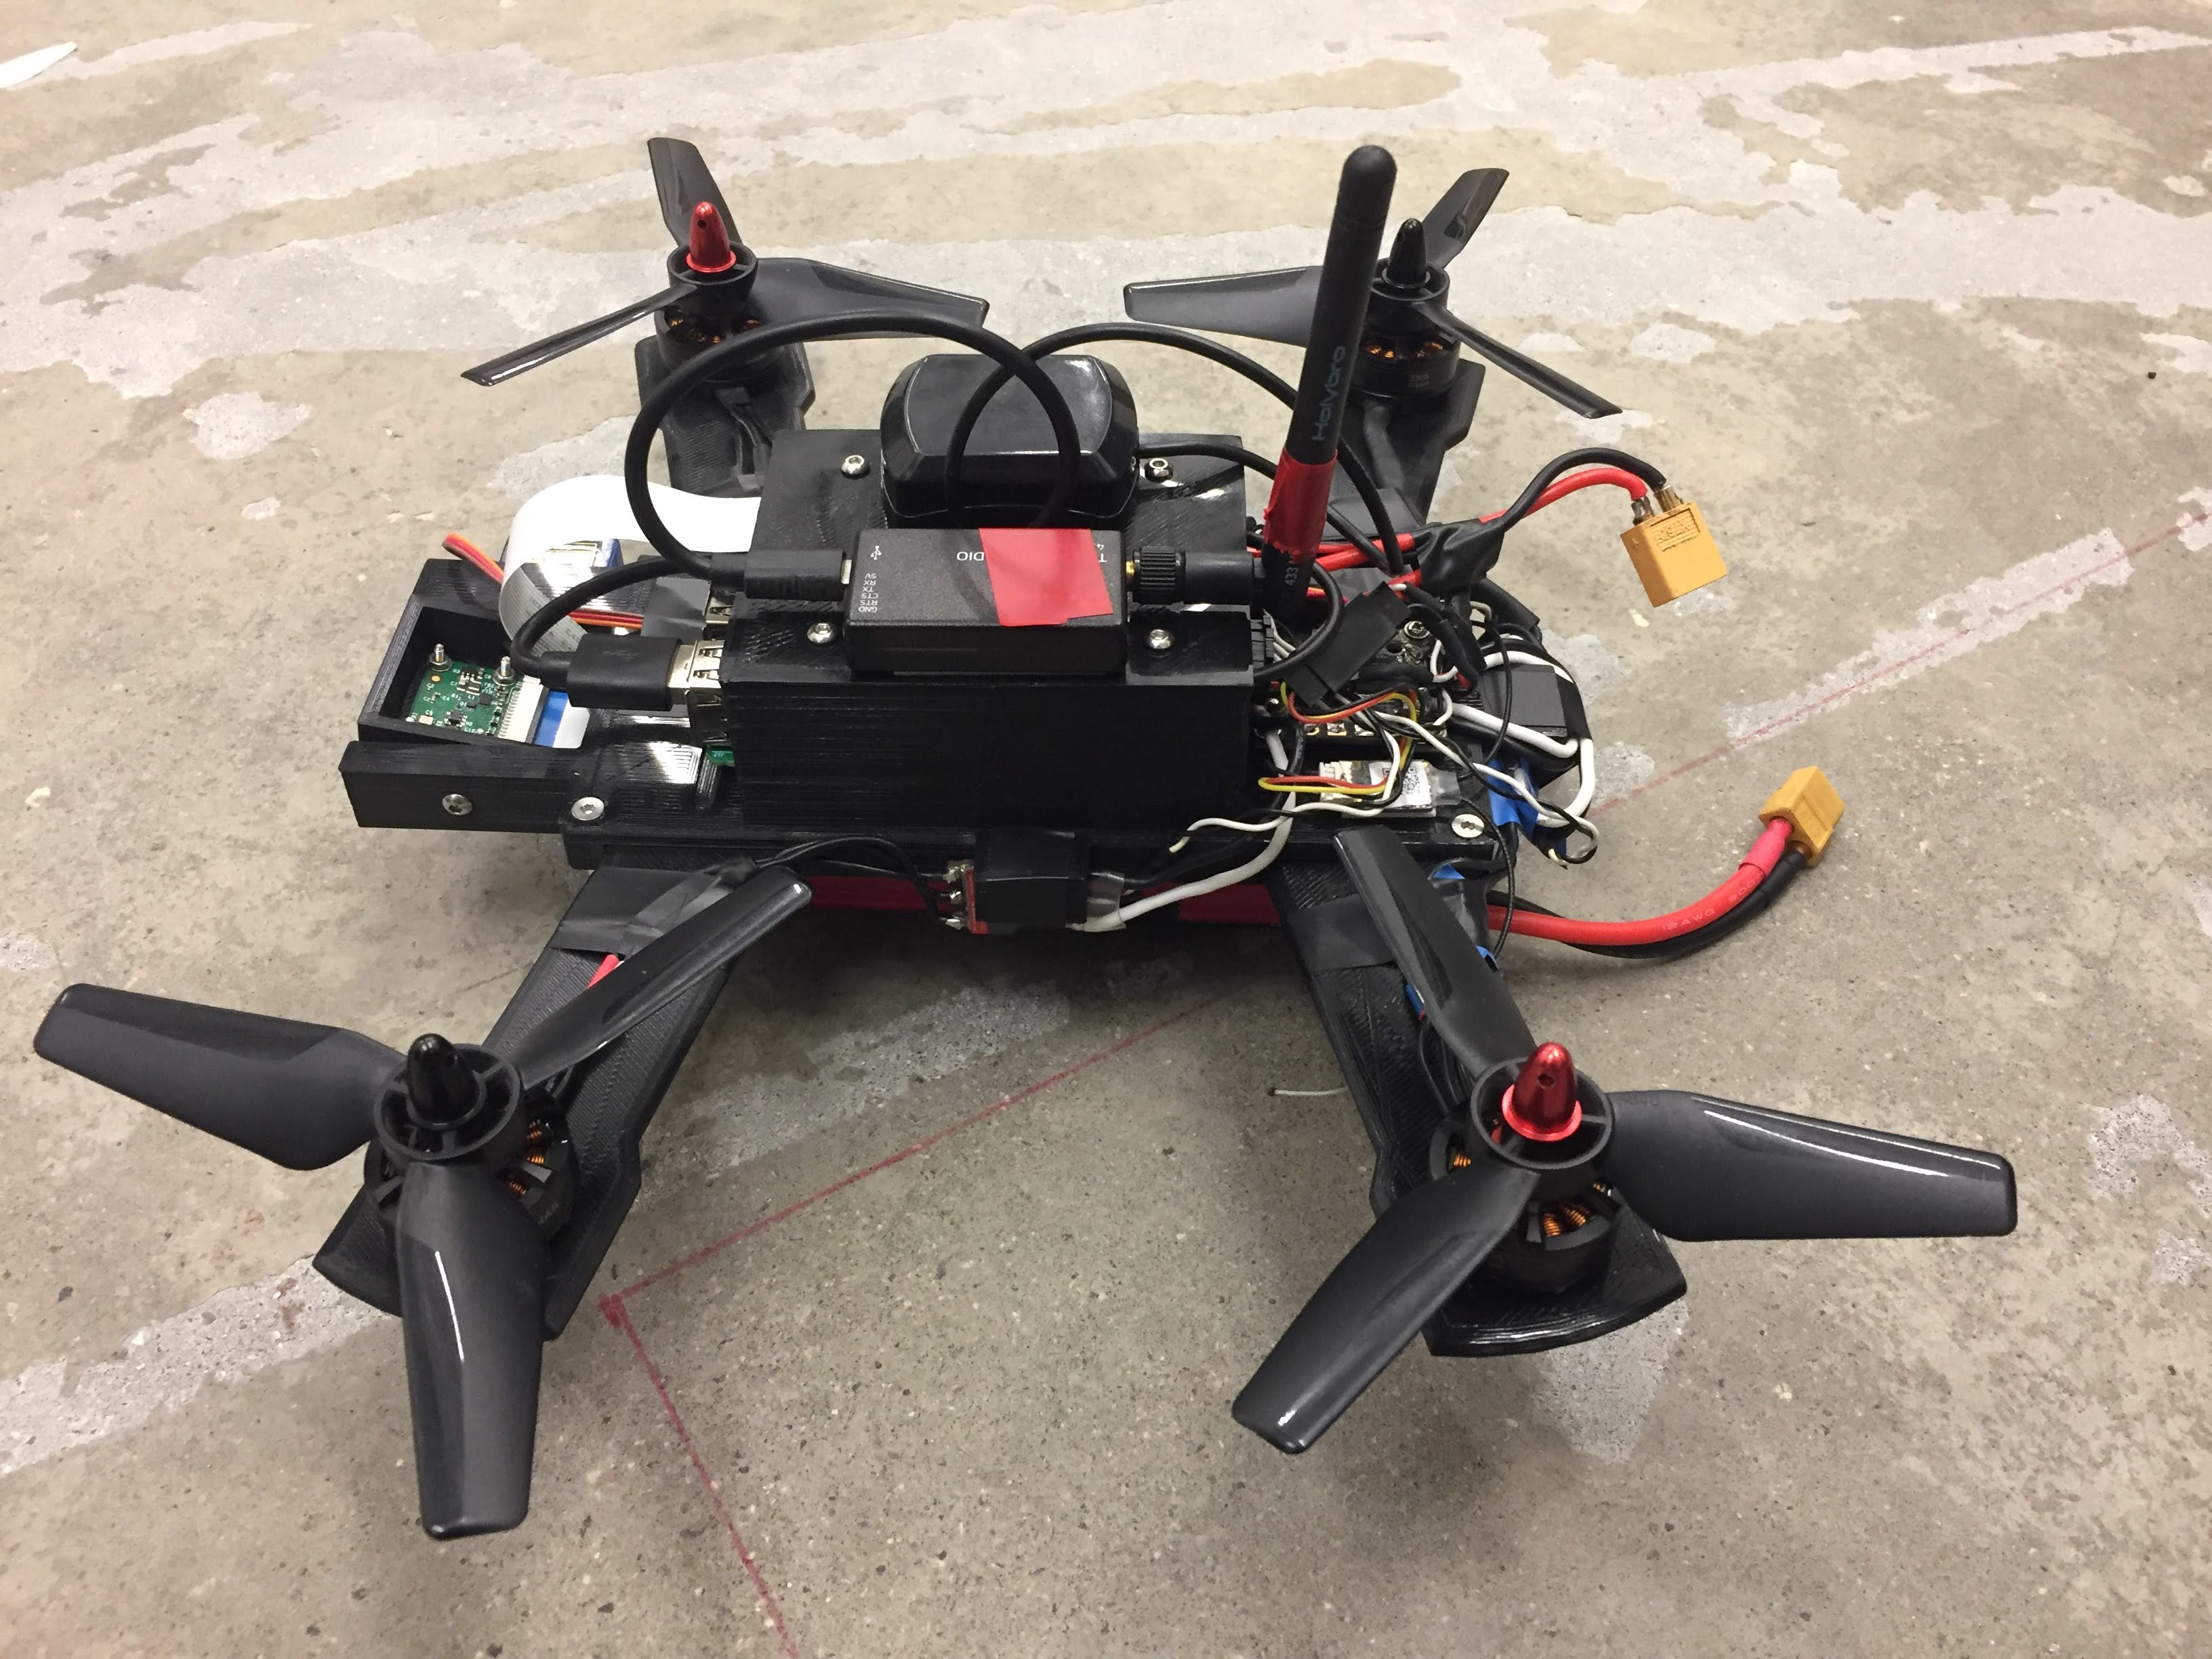
\includegraphics[width=\columnwidth]{images/drone_assembled.jpg}
    \caption{The assembled drone.}
    \label{figure:drone_assembled}
\end{figure}